%!TEX root = ../main.tex

\chapter{Introduction}
\label{chp:intro}

The term \ac{NTNs} refers to a category of networks where at least one link is routed via an aerial or space-borne vehicle such as \ac{HAPs}, \ac{UAVs} or telecommunication satellites.

\section{The focus on non-terrestrial networks}
The Third Generation Partnership Project \footnote{\href{https://www.3gpp.org}{\texttt{3gpp.org}}} (3GPP), the standardization body developing protocols for mobile communication networks, recently put a great emphasis on the importance of the integration of different access technologies along with the existing terrestrial mobile telecommunication infrastructure \cite{3gpp-tr-21.917}.

The envisioned future for mobile communications, starting with the already established 5G \ac{NR} and expanding with the new sixth-generation cellular networks (6G), foresees the integration of a non-terrestrial component. The latest \ac{3GPP} releases (Rel. 17 and Rel. 18) require 5G and 6G networks to be able to provide non-terrestrial satellite access complementing the already existing terrestrial access technologies \cite{overview-rel-17-18-saad} \cite{5g-nr-communication-geo-leo-maattanen}.

\section{Limitations of terrestrial networks}
The following paragraphs present a few scenarios where terrestrial networks have some limitations, and \ac{NTNs} can be used to provide connectivity.

\subsection{Remote places}
While \ac{TN} make the well-established foundation of today’s mobile communication infrastructure, their own nature poses some intrinsic limitations to their deployment in certain scenarios, especially in rural and remote areas. Conditions such as harsh terrain and geographical impediments act as natural barriers to the deployment of terrestrial infrastructure. Moreover, ground infrastructure requires the presence of an already established reliable power grid, driving up the costs that telecommunication companies would have to sustain.
The population density is often low in remote and rural places, so the already high infrastructure cost will hardly pay for itself, making this kind of market even more unattractive to private investors and further limiting the possibility for the people living there to access a resource which is becoming increasingly more important.

As studied and documented in \cite{6g-challenge-opportunity-base-pyramid}, the issue of an inadequate broadband coverage in rural regions is an enormous challenge, but also a great opportunity to kick-start the economy of currently underdeveloped countries, promoting a more fair access to the internet and alleviating the problem of digital divide between different parts of the world.

\subsection{Redundancy}
Another limitation of the current terrestrial infrastructure is the lack of redundancy and robustness against natural disasters. Extreme events such as earthquakes, fires and floods, but also deliberate behaviors such as targeted attacks by terrorist organizations and sabotages can disrupt the connectivity even for a long period of time, causing significant economical damage and hindering the already difficult rescue efforts, potentially leading to loss of lives.

The simple installation of a greater number of base stations is not a viable solution because they would all share the same weaknesses.

In this scenario, \ac{NTNs} can act as redundant access methodology to decrease downtimes of terrestrial infrastructure, provide emergency communication services and also additional capacity when required.
Fig. \ref{fig:multiple-connectivity}, courtesy of \cite{3gpp-tr-38.811}, shows a scenario where terrestrial and non-terrestrial access technologies are used in a transparent fashion to access the network. 

\begin{figure}[ht]
    \centering
    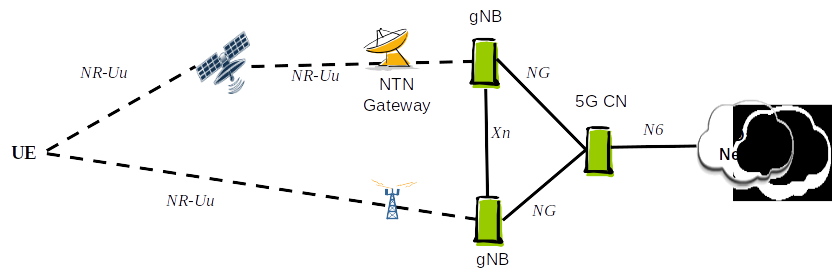
\includegraphics[width=0.7\textwidth]{res/multiple-connectivity.png}
    \caption{Trasnparent use of multiple radio access technology \cite{3gpp-tr-38.811}}
    \label{fig:multiple-connectivity}
\end{figure}

\subsection{Long distances and sensors}
Remote equipment, offshore plants and distribution grids will also benefit from the research carried out in this field, since providing terrestrial connectivity in those scenarios is a challenging task. The installation of an underwater optical fiber link to serve a single endpoint, such as an offshore power plant in the ocean, would bear a disproportional cost compared to the functions required, and maintenance would be another challenging and expensive task. 
The deployment of a non-terrestrial network would provide connectivity on a global scale, therefore allowing internet access in isolated places without the need for a dedicated connection.

Consider now the problem of connecting of a number of sensors placed in a large area. When distances are large, solutions may either be the densification of radio stations or the use of a lower frequency in order to have a less severe propagation loss. However, those approaches have their downsides and are not always feasible. In this case, the large coverage area of \ac{NTNs} will undoubtedly be useful to provide internet connection \cite{performance-ntn-support-iot-wang}.

\paragraph{} Other scenarios where \ac{NTNs} can become useful in overcoming the limitation of their terrestrial counterpart are well described in \cite{ntn-6g-era-challenges-giordani} and \cite{potential-multilayered-nierarchical-ntn-wang}.

\section{Satellite types}
\label{sec:satellite-types}
Satellites are divided in three different categories depending on their orbiting altitude: \ac{GEO}, \ac{MEO} \ac{LEO} satellites. Each one has its own characteristics, as briefly described below. Fig. \ref{fig:satellite_coverages} illustrates the different orbiting altitudes as well as the approximate coverage area for each orbit.


\begin{figure}[ht]
    \centering
    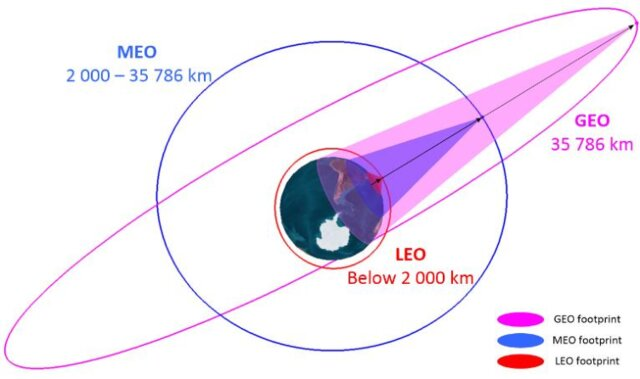
\includegraphics[width=0.7\textwidth]{res/satellite-coverages.jpg}
    \caption{Approximate coverage areas for satellites at different orbits\cite{sustainable-sat-com-6g}}
    \label{fig:satellite_coverages}
\end{figure}

\subsection{GEO satellites}
Orbiting at 35.786Km, \ac{GEO} satellites appear stationary since their period is the same as the Earth rotation period. This vastly simplifies the tracking for the ground equipment, since once the position of the \ac{UE} is known, the relative position of the satellite is known, too.

\paragraph{Advantages}    
Since \ac{GEO} satellites are geostationary, continuous coverage to a designated area can be provided using as little as a single satellite, while the use of non-\ac{GEO} satellites would require the deployment of a constellation, which is both more complex and more expensive. Almost full coverage of the terrestrial globe can be achieved using only three equally spaced satellites \cite{types-of-orbits-esa}.

As shown in Fig. \ref{fig:satellite_coverages}, their high altitude creates a large cell footprint. While the deployment cost of a single \ac{GEO} satellite is higher than both \ac{MEO} and \ac{LEO} ones, the cost per coverage area is overall lower.

\paragraph{Disadvantages}
The disadvantages of \ac{GEO} satellites are mainly linked to the large distance with the \ac{UE}: the transmission power and the antenna gain have to be higher to account for the greater propagation losses, and the propagation delay of the signal adds about 120ms to the overall latency. This means that if the \ac{UE} sends a request to a server at $t=0$ through a \ac{GEO} link, the packet will be received by the destination node at least at $t=240$ms. The response will finally reach the \ac{UE} after at least $480$ms, without considering any delay related to medium access requests, packet transmission times and processing delays.

In addition to the positive aspects previously discussed, the larger cell footprint also brings some downsides with it. Due to the vast area, a single satellite will be serving a massive number of users, so the total available capacity will have to be shared between a bigger number of actors, and the throughput experienced by each of them will be reduced. Solutions have been proposed and are currently in early stage in order to provide more capacity, such as the use of higher frequency bands towards Ku, K and Ka as depicted in Fig. \ref{fig:satellite-bands} and beamforming \cite{advances-comm-sat-sys}.
Moreover, the high number of users leads to a large rate of initial access requests, with the possibility of channel saturation as described in \cite{3gpp-tr-38.811}.

\begin{figure}[ht]
    \centering
    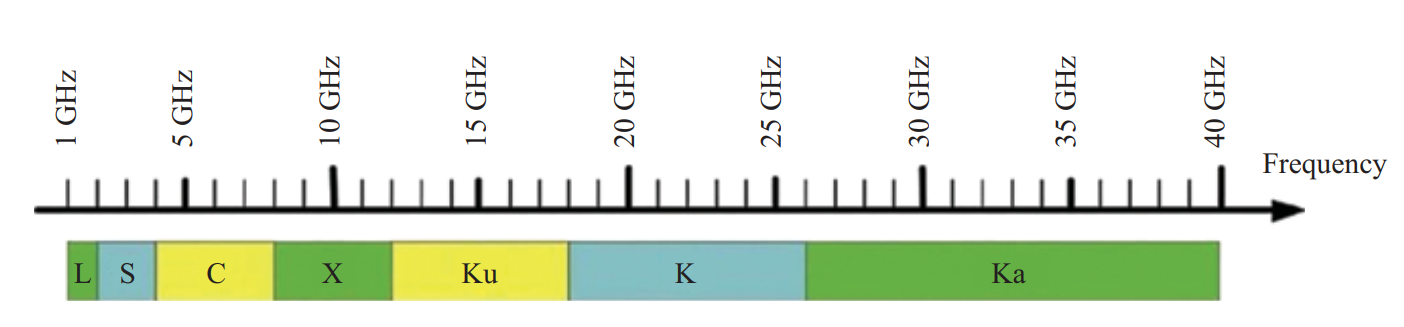
\includegraphics[width=0.7\textwidth]{res/satellite-bands.png}
    \caption{Satellite spectrum bands allocation \cite{advances-comm-sat-sys}}
    \label{fig:satellite-bands}
\end{figure}

\subsection{MEO satellites}
\ac{MEO} orbit is comprised between \ac{LEO} and \ac{GEO}, therefore all satellites orbiting between 2000Km and 35.786Km are considered \ac{MEO}. This vast orbital space is mainly used by navigation systems such as GALILEO \cite{types-of-orbits-esa}.

The propagation delay can vary a lot depending on the altitude, but is generally larger than \ac{LEO} and smaller than \ac{GEO}. The same point can be made regarding the cell size and number of served users. 

\ac{MEO} satellites do require a constellation in order to provide continuous coverage over a designated area, since they are not geostationary. The numerology of the constellation, however, is smaller than the one required for \ac{LEO} satellites, since each platform can serve a larger area.

\subsection{LEO satellites}
Orbiting below the altitude of 2.000Km, \ac{LEO} satellites are the most promising solution in the realm of \ac{NTNs} for a number of reasons hereby discussed.

\paragraph{Advantages}
The lower altitude entails a shorter propagation delay, on the order of 6ms, and the smaller coverage area of each satellite depicted in Fig. \ref{fig:satellite_coverages} means that the total number of users that need to be served is smaller. This also enables the use of higher frequency bands with smaller antennas, since the experienced path loss is smaller compared to \ac{GEO} satellites. This in turn allows for higher throughput, as detailed in \cite{satellite-communication-mmwave-giordani}.

\begin{figure}[ht]
    \centering
    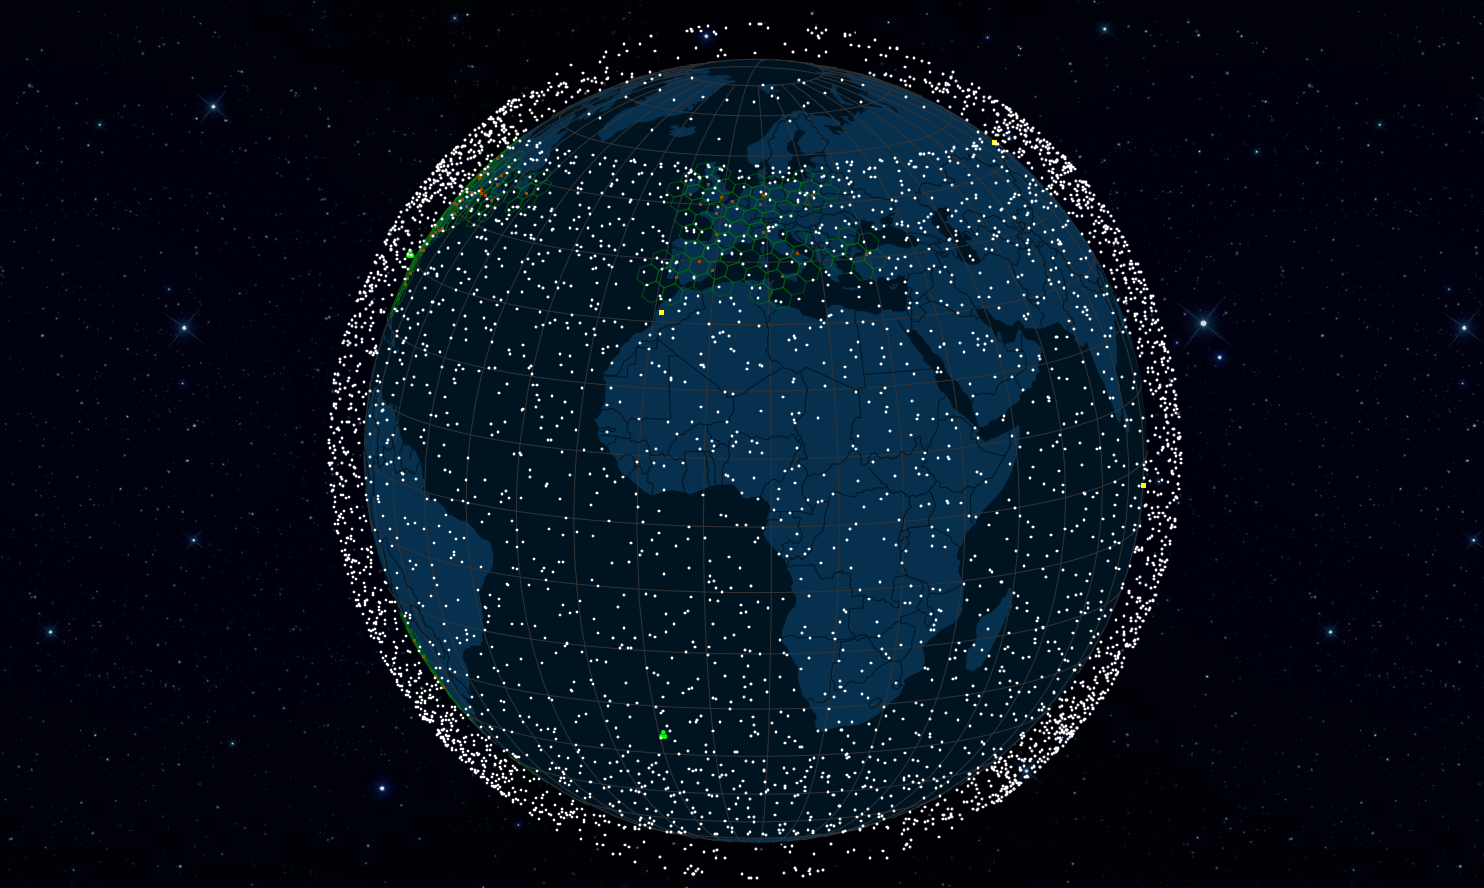
\includegraphics[width=0.7\textwidth]{res/starlink-constellation.png}
    \caption{Starlink constellation as July 2024. Source: \href{https://satellitemap.space/}{\texttt{satellitemap.space}}}
    \label{fig:starlink_constellation}
\end{figure}

\paragraph{Disadvantages}
The cost per satellite is significantly smaller than \ac{GEO} and \ac{MEO} satellites. However, given that they are not geostationary, a large constellation is needed to provide a continuous service, driving up the deployment costs significantly. As an example of those constellations, Fig. \ref{fig:starlink_constellation} depicts the \ac{LEO} satellites employed by Starlink\footnote{Starlink is a satellite internet constellation operated by Starlink Services, LLC, a wholly-owned subsidiary of American aerospace company SpaceX.}, with 4.808 units in service at the time of writing\footnote{Source: \href{https://satellitemap.space/}{\texttt{satellitemap.space}}}.

The small coverage area of each satellite means that more terrestrial gateways have to be deployed, and inter-satellite links have to be implemented in satellites if coverage over the oceans is required. This adds up to the already high constellation deployment costs.

\subsection{Multilayered networks}
The aforementioned solutions are not to be considered mutually exclusive. In fact, the multitude of possibilities that their combinations offer open to the study of various different scenarios, as detailed in \cite{potential-multilayered-nierarchical-ntn-wang}.
\todo{add descriptions and ideally images of multilayered hierarchical networks}.

\section{Types of payloads}
When implementing a non-terrestrial network, an important parameter that can be decided is the type of payload to use.
\subsection{Bent pipe payoad}
This is the most simple approach, where the role of the satellite is simply to repeat the signal received from the \ac{UE} on the groud towards the terrestrial gateway. Configurations such as the one depicted in Fig. \ref{fig:ntn-bent-pipe} go by the name of bent pipe and are characterized by the presence of a terrestrial g-NodeB, while the satellite has the sole purpose of providing a link with the \ac{UE} in a transparent way.

While such solutions are by far the simplest ones, the main drawback is the even longer propagation delay, since communications between users served by the same satellite would also have to be routed through the terrestrial gateway, increasing the latency by at least $2\tau_p$.
This scenario also poses high bandwidth requirements the feeder link, since all the traffic must necessarily pass through the main link.
Other solutions are smarter and are able to route at least part of the inbound traffic autonoumously.

\begin{figure}[ht]
    \centering
    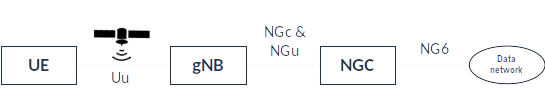
\includegraphics[width=0.7\textwidth]{res/ntn-bent-pipe.png}
    \caption{NTN with access network based on satellites with bent pipe payload \cite{3gpp-tr-38.811}}
    \label{fig:ntn-bent-pipe}
\end{figure}

\subsection{On-board g-node b}
A slightly more sophisticated approach foresees the installation of g-NodeB capabilities directly on the satellite. This has the benefit of reducing the experienced latency in some cases, and reduce the utilization of the feeder link. Certain protocols, designed to terminate at the \ac{gNB}, can also reach their designated endpoint without necessitating to be routed back to the gateway.

Figure \ref{fig:ntn-gnb-onboard} from \cite{3gpp-tr-38.811} shows the architecture of a \ac{NTN} using access network based on satellites with \ac{gNB} on board as payload.

\begin{figure}[ht]
    \centering
    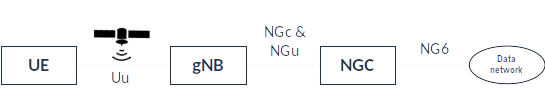
\includegraphics[width=0.7\textwidth]{res/ntn-bent-pipe.png}
    \caption{NTN with access network based on satellites with gNB payload \cite{3gpp-tr-38.811}}
    \label{fig:ntn-gnb-onboard}
\end{figure}

\subsection{Inter-satellite links}
The served area of each satellite decreases with its altitude, therefore lower-orbiting platforms cannot provide long-distance links on their own, and their characteristic of not being geostationary further complicates the matter.

In order to provide global coverage, the aid of a high number of gateways scattered in the designated coverage area is required to keep the connection with each member of the constellation as it sweeps the earth surface. Another solution requires the usage of \ac{ISL} as some sort of backbone connecting the constellation with the gateways. Satellites that do not have a gateway in sight can use \ac{ISL}s to forward their traffic to satellites illuminated by feeder links, therefore providing global connection. 

\section{Currently available commercial solutions}
Commercial solutions for satellite-based internet access have been available since a long time. However, the majority of internet service providers have been using \ac{GEO} satellites, orbiting at a height of 35.786 km, therefore presenting all the limitations discussed in \ref{sec:satellite-types}. The distance that the signal  to travel offering limited throughput and large delays. While \ac{LEO} constellations (400 km to 2.000 km) have proven to be a valid alternative, providing higher throughput and lower latency \cite{main-features-5g-nr-ntn-yun}, they have the drawback of an increased Doppler shift due to their high speed relative to ground \cite{satellite-communication-mmwave-giordani}, and there is still no international standard with regard to the communication protocols to use. 
\todo{expand}

\paragraph{}
It is clear that the future of mobile networks envisioned by \ac{3GPP} embraces \ac{NTN}s, and considerable work has to be done. Research will bear a high impact towards a more connected, equal opportunity world. 
